\RequirePackage{lineno}
\documentclass[aps,pt14,superscriptaddress,showpacs,floatfix,nofootinbib]{revtex4}
%preprint
\usepackage{graphicx}
%\linenumbers
\begin{document}
\begin{center}
\large\bf{Simulation of 3D-Silicon sensor with a Low-Gain Avalanche Diode (LGAD) for a fast timing pixel detector}
\end{center}
%\begin{center}
%Wei-Ming Yao
%\end{center}
\section{abstract}

Presently, the silicon
pixel detector either has no proper timing or has proper timing, but with a
pixel size at the mm level, too large for precision tracking.
The 3D-sensor has excellent spatial resolution and it could potentially be a fast timing detector with a timing
resolution of $\approx$30~ps as demonstrated by the recent study.
In this study, we present some preliminary results on the 3D-LGAD sensor based TCAD simulation, which
could improve the signal-to-noise ratio to achieve a better timing resolution.
We aim to develop a truly 4-D silicon pixel detector with 3D sensor with both a spatial
resolution of $\approx 10~\mu m$ and a timing resolution of $\approx$30~ps
that  will open a new era for precision tracking, reducing pile-up
events and particle identification for the future colliding experiment.

\section{Introduction}

Silicon detectors provide at present the most precise tracking for charged
particles in high energy physics experiments. They have an excellent space
point resolution and granularity to cope track separation in dense jets and
hits from the high luminosity beam related background.
The recent developments of a new silicon sensor based on Low-Gain Avalanche
Diodes (LGAD) provide a significantly enhanced capability to measure
track arrival times with a resolution of $\approx$30~ps, which allows for tracks to be 
separated from pile-up events and particle identification. Presently, the silicon
pixel detector either has no proper timing or has proper timing, but with a  
pixel size at the mm level, too large for precision tracking.

The 3D sensor was first introduced in 1997 by S. Parker et al.~\cite{Parker:1996dx}.
It decouples the electrode distance from the active substrate
thickness providing several superior features, which makes it more radiation hard,
and fast charge collection compared to the planar sensor.
The first application of 3D sensors was successfully installed for
the ATLAS Insertable B-Layer (IBL), and the sensor design has been
further improved for the HL-LHC developed by CNM~\cite{Pellegrini:2008zza}
and FBK~\cite{Sultan:2016vzg}.
The recent study with a small cell 3D sensor demonstrated that it
could potentially be a fast timing detector with a resolution
of $\approx$30~ps~\cite{Kramberger:2019ygz}.

The idea proposed here is to develop a new type of 3D sensor with internal
charge multiplication by adding a thin low-resistivity diffusion gain layer surrounding
the readout electrode with a highly doped implant.
The thin layer will enhance the high electric field to cause multiplication of
charge carries that transverse the region, which will improve the signal-to-noise ratio to
achieve a timing resolution better than $\approx$30~ps.
From a simple calculation, the gain is similar to what obtained
in the planar LGAD detector.

\section{LGAD}

The planar LGAD detector has a gain layer that contains high electric field to
cause multiplication of charge carries that transverse the region.
The gain is achieved by raising the electric field high enough to enable the
charge carriers to create secondary ionization during the charge collection process.
The main difference to standard APD detectors are the low gain
required to detect high energy charged particles in the thin sensors.
With the low gain these sensors can be very thin to have a fast drift time
and have enough signal-to-noise ratio to achieve good time resolution.

The fast timing detector has been studied extensively for HL-LHC upgrades where the
excellent time resolution coupled with good spatial resolution can help to
reduce pile-up events. ATLAS has recently proposed to use the High Granularity
Timing Detector (HGTD) in the forward region and CMS is considering adding
a timing layer in the barrel region with SIPM for photon detection, while using HGTD
in the forward region. In both cases, the timing detector is 
limited to have a pad size of 1 mm x 1 mm with a time resolution of $\approx$30~ps, but this 
size is too large to be useful for precision tracking.

The timing resolution is determined mainly by contributions from time walk and noise
jitter. The time walk contribution is usually minimized by using Constant Fraction
Discrimination (CFD) or determining time of the signal crossing fixed threshold.
The jitter contribution is determined by the rise of the signal at the output of
the amplifier and noise level. The timing resolution can be improved with larger
gain as well as with thin detectors since both increase the slew-rate of the amplifiers.
However, the time walk is dominated by Landau fluctuations due to
the non-uniform charge deposition within the sensors, especially for LGADs where
electrons need to reach the gain layer to multiply

\section{TCAD simulation}
The simulation is performed using the Synopsys Sentaurus TCAD simulation toolkit
to understand the elctrical behavior for the proposed 3D-LGAD sensor. 
We use the same TCAD setup for the ATLAS IBL 3D pixel detector study and
simply add an extra thin low-resistivity p+ doping gain layer of 3 $\mu$ thick
surrounding the n+ readout electrode. The IBL 3D pixel cell consists of two connected n+ 
readout electrodes (2E) surrounded by eight p+ electrodes with a size of 50x250x230 $\mu m^3$
as shown in Fig.~\ref{fig:ibl-3d}. We use a reduced red rectangle area in TCAD simulation to save time 
by taking the advantage of 8-fold symmetry of IBL 3D pixel. 

\begin{figure}[hbtp]
\begin{center}
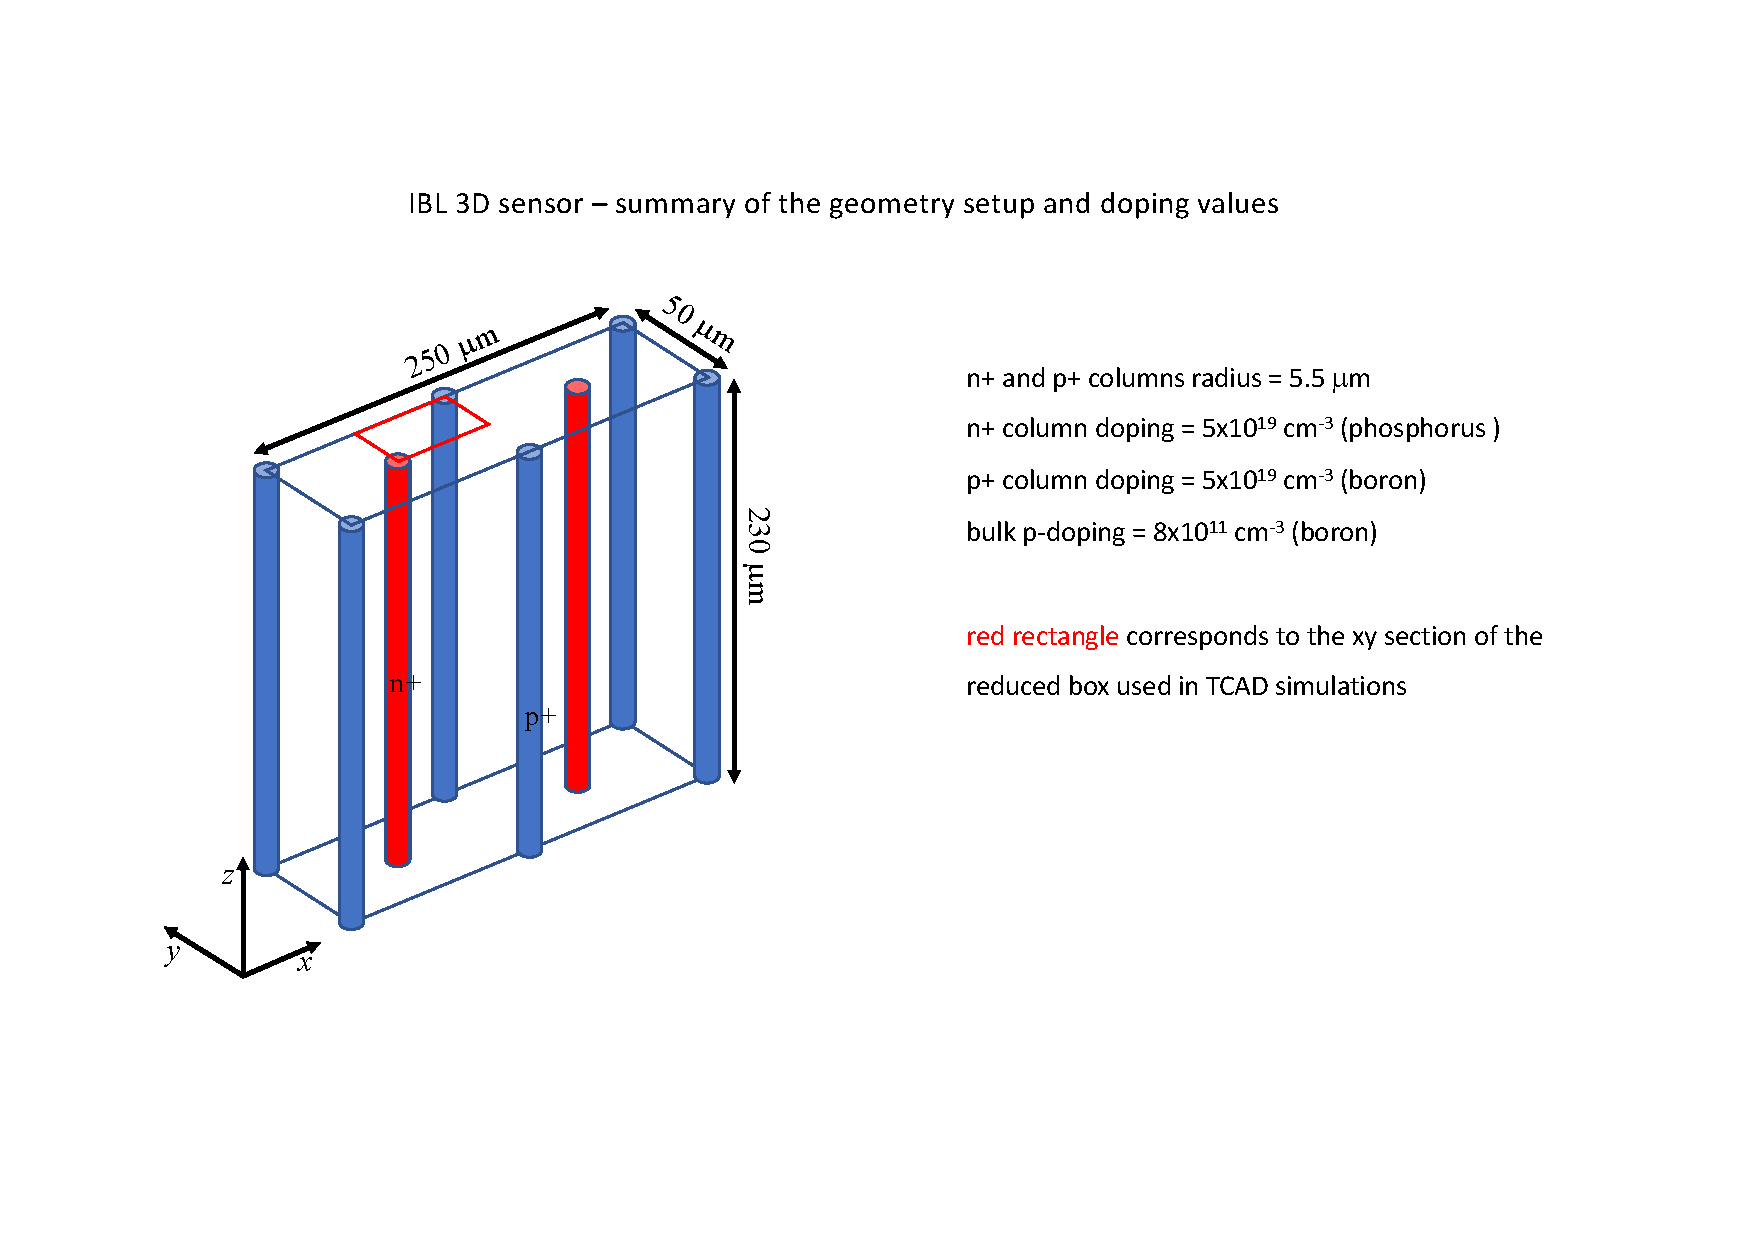
\includegraphics[width=0.35\textheight,keepaspectratio]{figures/IBL3D_setup.pdf}
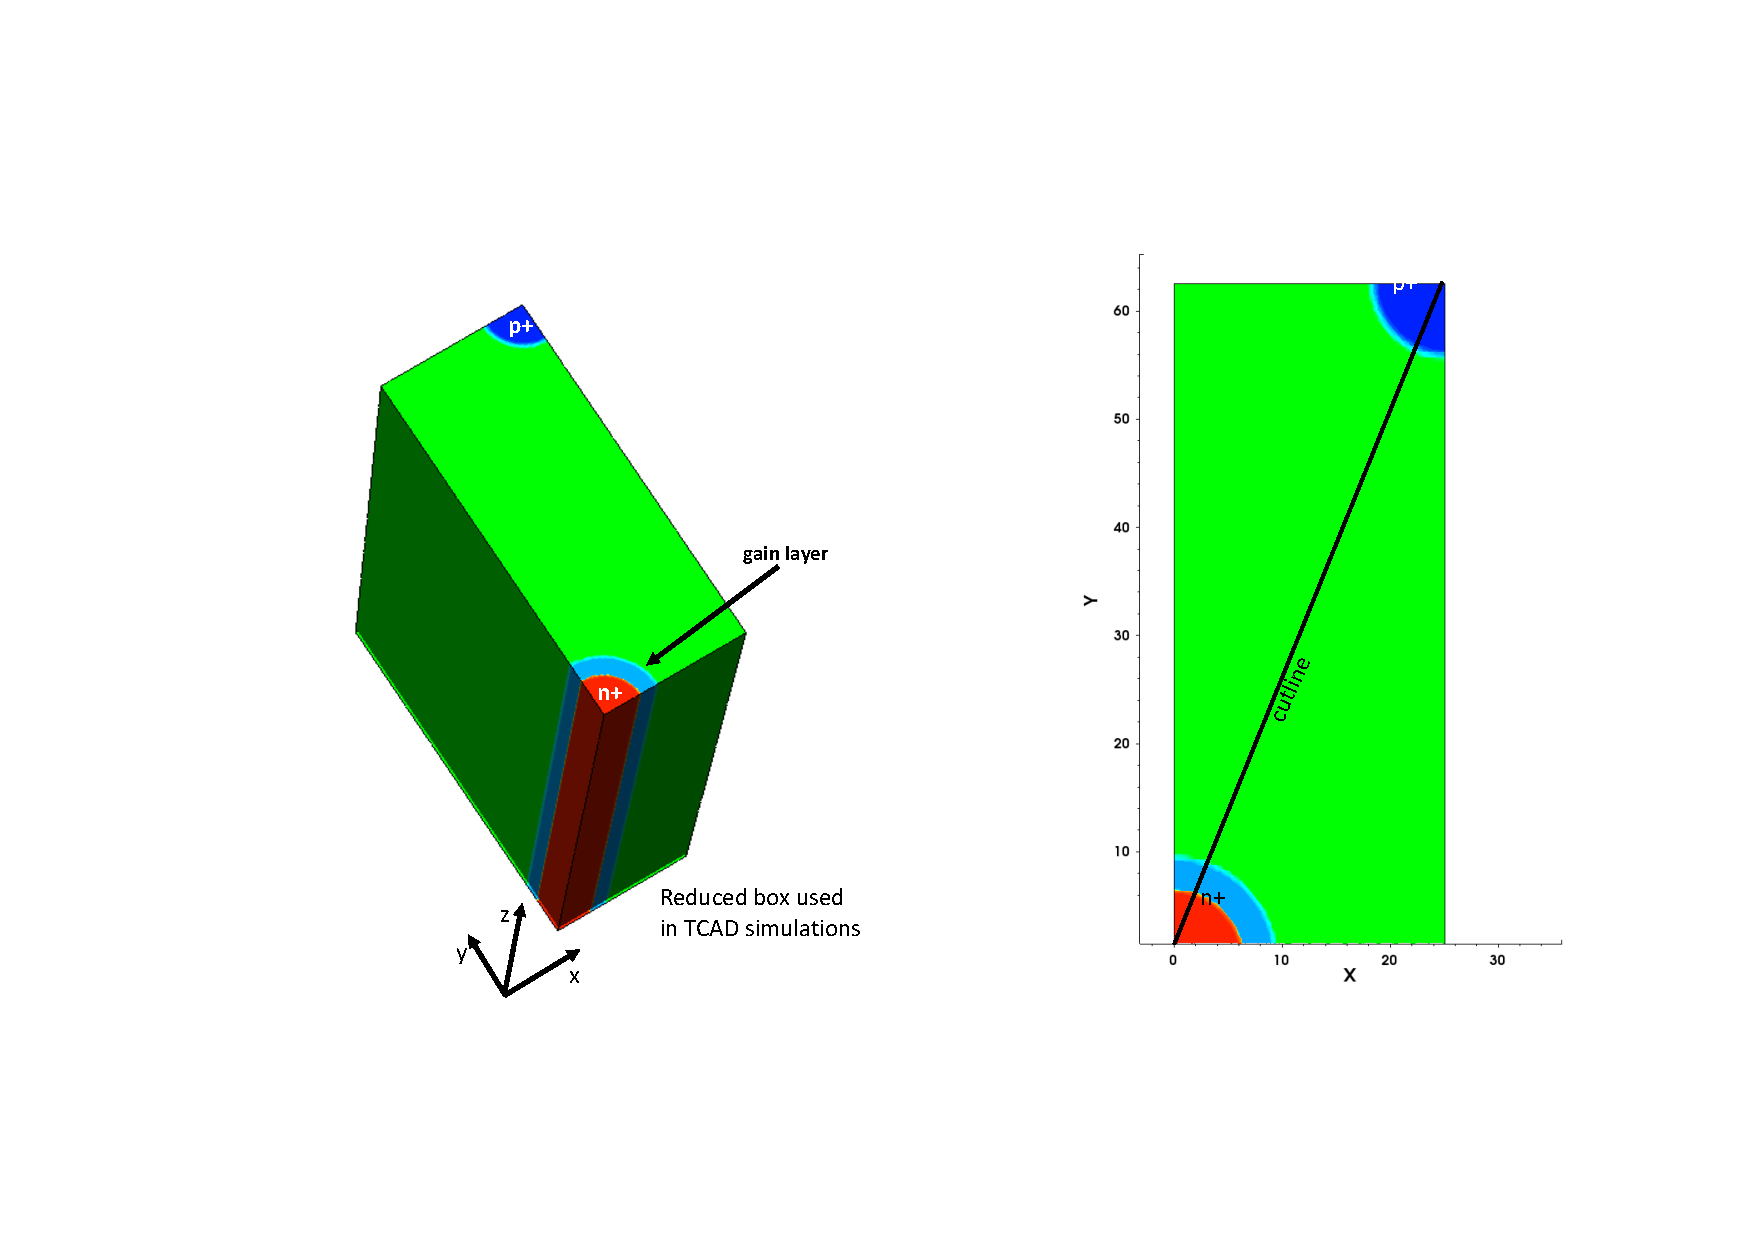
\includegraphics[page=1,width=0.35\textheight,keepaspectratio]{figures/IBL3D_250x50x230_withGainLayer_efield.pdf}
\caption{A schematic view of IBL 3D pixel sensor (right) and the reduced box used in TCAD simulation 
(right).\label{fig:ibl-3d}}
\end{center}
\end{figure}

\subsection{Electric properties}    
We have considered different values for the p+ doping
concentration of the gain layer (ranging from $10^{14}$ to $10^{16}$ cm$^{-3}$).
For higher gain layer doping concentrations, breakdown takes place before the depletion. 
Fig.~\ref{fig:efield} shows the electric field maps and projection along the diagonal line 
between n+ and p+ electrodes with a bias voltage of 100 V for the unirradiated sensor. 
The results for irradiated sensor at fluence of 1.0e 15 neq/cm$^2$ are also studied 
and they do not display any significant change. 
As the gain layer doping is increased, the electric field shows expected increase in the gain layer region.
  
\begin{figure}[hbtp]
\begin{center}
\includegraphics[page=2,width=0.5\textheight,keepaspectratio]{figures/IBL-3DwithGainLayer_20190610_toWeiming.pdf}
\caption{The projection of the electric field along the diagonal line between n+ and p+ electrodes with a bias voltage of 100V
in a log-scale (left) and a linear-scale (right).~\label{fig:efield}} 
\end{center}
\end{figure}

The current-voltage (I-V) curves and the capacitance-voltage (1/C$^2$-V) curves are also checked for 
different doping densities of the gain layer (GL) as shown in Fig.~\ref{fig:IV-C} with non-irradiated sensor.
There is a prefect correspondence between the jumps in the I-V curves and the jumps in 1/C$^2$ - V curves, which 
should be a clear signature of depletion.  
Note that the current values are so small because they correspond to the
current for only the reduced box used for the TCAD simulation; for
comparison to a practical measure they should be rescaled by taking into
account the number of the sensors in a module.

\begin{figure}[hbtp]
\begin{center}
\includegraphics[page=3,width=0.35\textheight,keepaspectratio]{figures/IBL-3DwithGainLayer_20190610_toWeiming.pdf}
\includegraphics[page=4,width=0.35\textheight,keepaspectratio]{figures/IBL-3DwithGainLayer_20190610_toWeiming.pdf}
\caption{The curves for I-V (left) and 1/C$^2$-V (right) are shown for the GL with different doping 
densities.\label{fig:IV-C}}
\end{center}
\end{figure}

\subsection{Charge collection and timing resolution} 

A Minimum Ionizing Particle (MIP) is simulated for charge collection using the TCAD simulation. Fig.~\ref{fig:box_points}
shows the sketch of the reduced sensor area with different positions marked for the MIP passing through perpendicularly. 
The simulation is done only for a 1 $\mu m$ thick slice for saving time since the electric field does not change much 
with sensor thickness and we expect the results obtained here should be rather consistent with those one would obtain with 
larger sensor thickness.

\begin{figure}[hbtp]
\begin{center}
\includegraphics[page=5,width=0.6\textheight,keepaspectratio]{figures/IBL-3DwithGainLayer_20190610_toWeiming.pdf}
\caption{The sketch of the reduced sensor area with different positions marked for the MIP passing through perpendicularly
in TCAD simulation.\label{fig:box_points}}
\end{center}
\end{figure}
 
Fig.~\ref{fig:drift1}-\ref{fig:drift5} show the current and collected charge at the readout electrode for 
hits at points of A, C, E, G, and I, at different bias voltages of 60, 100, and 200 V, and for increasing 
the GL doping values. The same scale is used in
all graphs, which allows to clearly appreciate the increase in current
and collected charge as the GL doping reach high values. A deposited
charge by MIP of 80 e (electron charge) per um were considered and
collected charge is expressed as charge fraction with respect to the
deposited one. In our case, since the sensor thickness is 1 um, a charge
fraction of 1 means a collected charge = 80 e. Note how collected charge
for GL doping near 7x10$^15$ cm$^-3$ becomes, because of avalanches, also
larger than 5 times the deposited charge.

\begin{figure}[hbtp]
\begin{center}
\includegraphics[page=6,width=0.5\textheight,keepaspectratio]{figures/IBL-3DwithGainLayer_20190610_toWeiming.pdf}
\caption{The currents and collected charges as a function of time are shown for different 
hit positions and bias voltages with no GL 3D sensor.\label{fig:drift1}}  
\end{center}
\end{figure}

\begin{figure}[hbtp]
\begin{center}
\includegraphics[page=7,width=0.5\textheight,keepaspectratio]{figures/IBL-3DwithGainLayer_20190610_toWeiming.pdf}
\caption{The currents and collected charges as a function of time are shown for different
hit positions and bias voltages with a GL doping density of 3x10$^{15}$ cm$^{-3}$.\label{fig:drift2}}
\end{center}
\end{figure}

\begin{figure}[hbtp]
\begin{center}
\includegraphics[page=8,width=0.5\textheight,keepaspectratio]{figures/IBL-3DwithGainLayer_20190610_toWeiming.pdf}
\caption{The currents and collected charges as a function of time are shown for different
hit positions and bias voltages with a GL doping density of 5x10$^{15}$ cm$^{-3}$.\label{fig:drift3}}
\end{center}
\end{figure}

\begin{figure}[hbtp]
\begin{center}
\includegraphics[page=9,width=0.5\textheight,keepaspectratio]{figures/IBL-3DwithGainLayer_20190610_toWeiming.pdf}
\caption{The currents and collected charges as a function of time are shown for different
hit positions and bias voltages with a GL doping density of 6x10$^{15}$ cm$^{-3}$.\label{fig:drift4}}
\end{center}
\end{figure}

\begin{figure}[hbtp]
\begin{center}
\includegraphics[page=10,width=0.5\textheight,keepaspectratio]{figures/IBL-3DwithGainLayer_20190610_toWeiming.pdf}
\caption{The currents and collected charges as a function of time are shown for different
hit positions and bias voltages with a GL doping density of 7x10$^{15}$ cm$^{-3}$.\label{fig:drift5}}
\end{center}
\end{figure}
 
The timing of arrival at 50\% of charge pulse height resolution (TOA50) is measured for these hits 
as a function of the distance from the n+ readout electrode in the transverse plane for different bias voltages and the GL 
doping densities.  The results are summarized in Fig.~\ref{fig:toamean}, which seems intuitive that the 
central hits have the lowest TOA.
Fig.~\ref{fig:toarms} shows the average mean of TOA50 and its RMS from 9 hit points as a function of the GL 
doping density for different bias voltage, respectively. The trend seems clear that the increase of TOA50 going 
from no GL to a higher GL doping density, which is caused by the slow drift of holes produced from the avalanches.
However, more studies are need to understand better the avalanche  process in TCAD simulation and the noise 
level of the front end electronics.   

\begin{figure}[hbtp]
\begin{center}
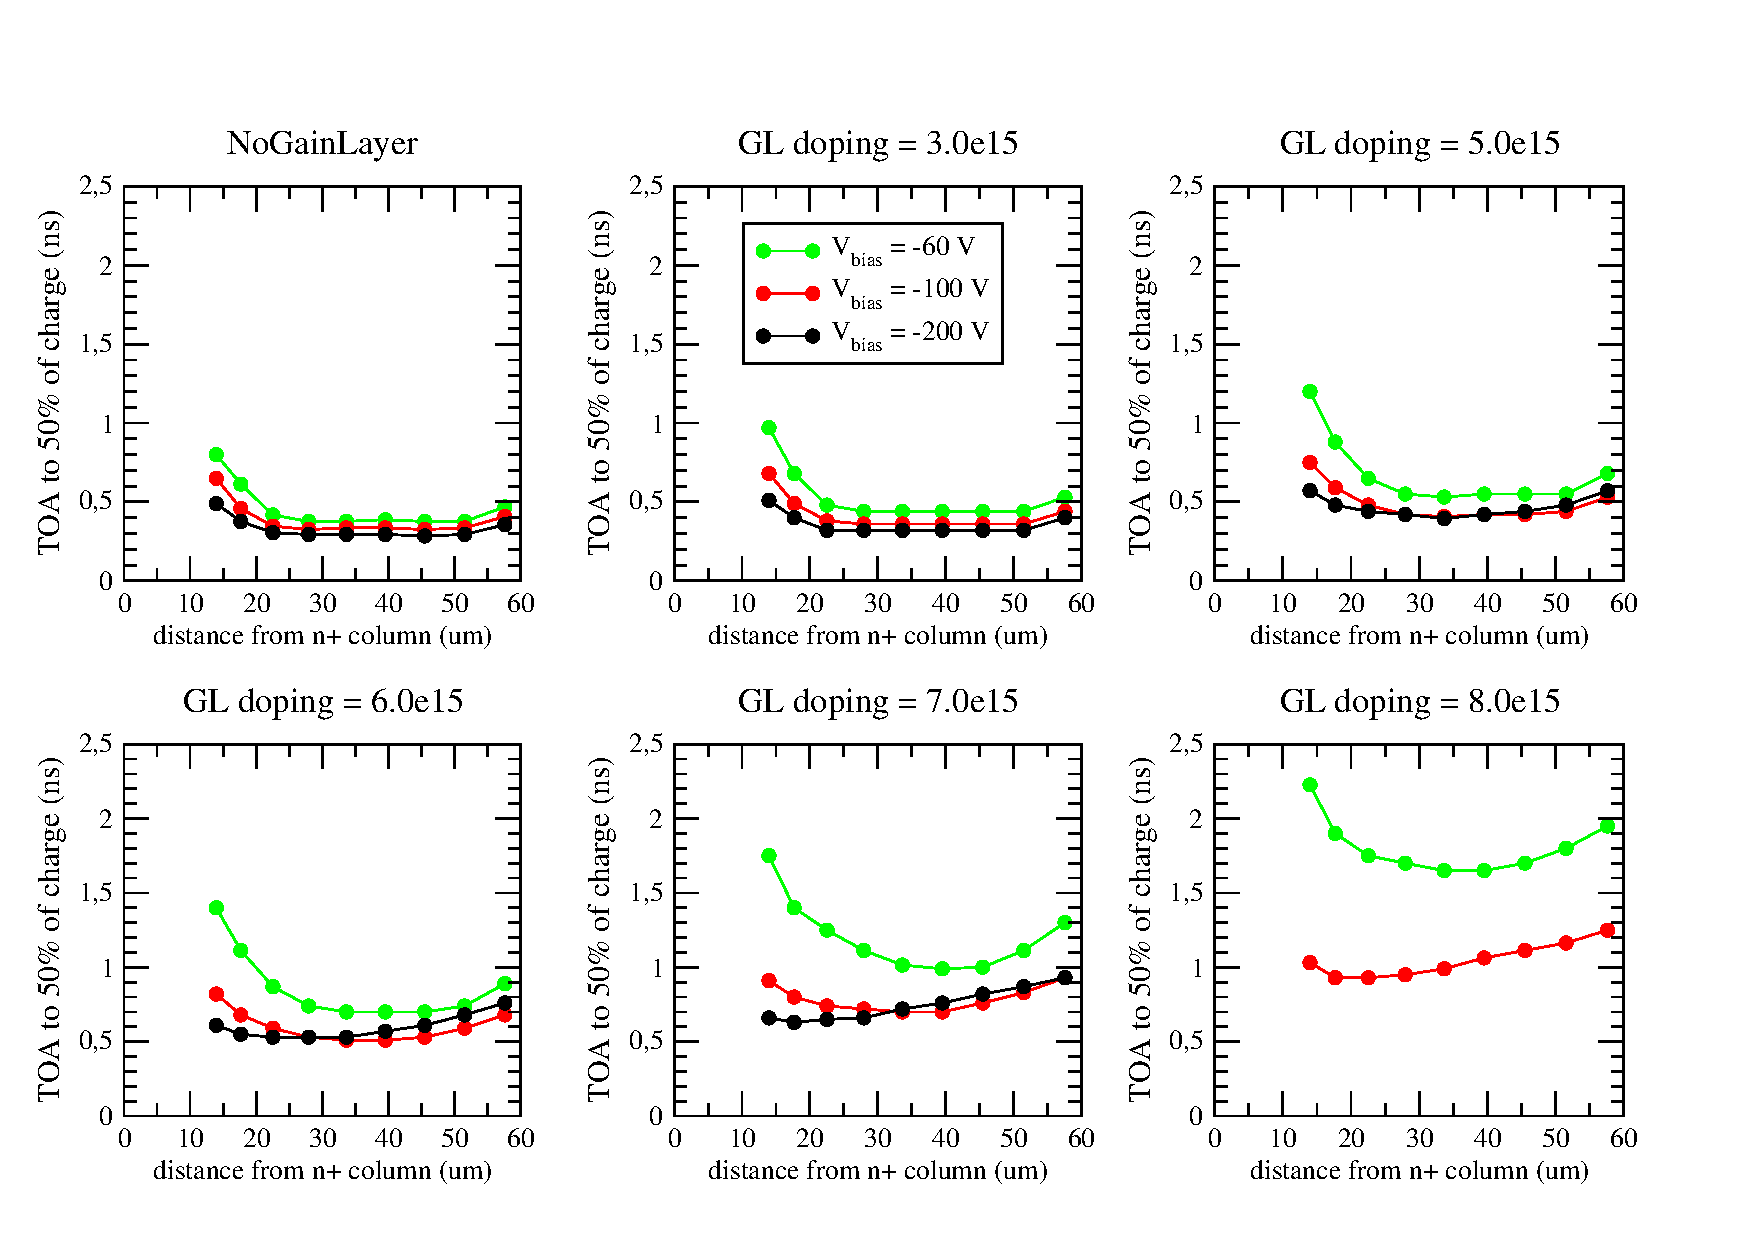
\includegraphics[width=0.5\textheight,keepaspectratio]{figures/MIP_Pulse_TOA50.pdf}
\caption{The measured TOA50 as a function of the distance between the hit position and the readout electrode in the
transverse plane for different bias voltages and the GL doping densities.~\label{fig:toamean}} 
\end{center}
\end{figure}

\begin{figure}[hbtp]
\begin{center}
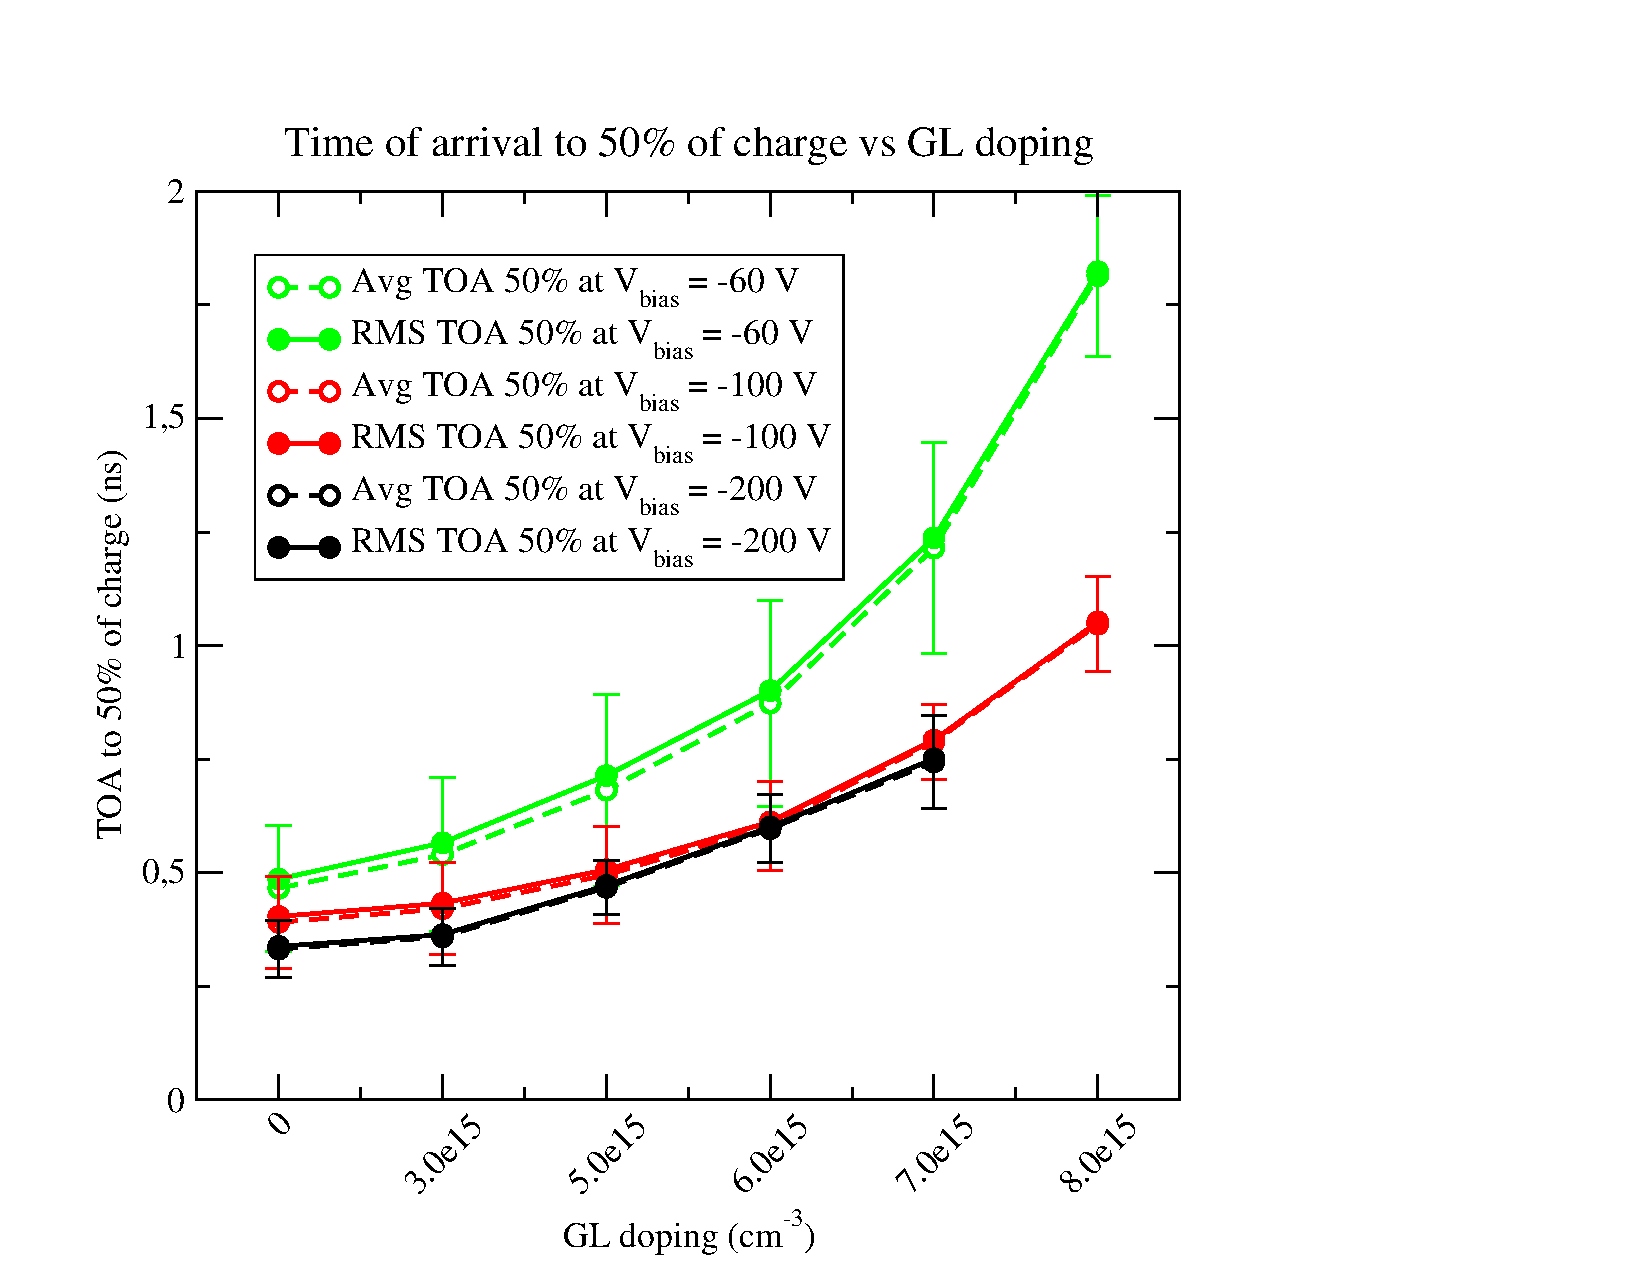
\includegraphics[width=0.5\textheight,keepaspectratio]{figures/ToA_vs_GLdoping.pdf}
\caption{The averages and RMS of 9 measured TOA50 as a function of GL densities and with different bias 
voltages.~\label{fig:toarms}}
\end{center}
\end{figure}

\section{Alternative studies with KDetSim} 

We also performed the studies using KDetSim~\cite{kdetsim} to simulate the charge collection in the proposed 3D-GLAD sensor.
The charge drift is simulated in steps with diffusion, impact ionization, and trapping also taken into account and  
the induced current is then proceeded with a transfer function of a front-end electronics with a shaping time of 1 ns. 
The results obtained from KDetSim are consistent with TCAD simulation. Fig.~\ref{fig:kdetgain} shows the projected 
electric fields (V/um) and the average charge collection gains for a MIP passing through randomly and perpendicularly 
to the detector as a function of GL doping densities and the bias voltage. Fig.~\ref{fig:kdettoa} shows the drift-time 
(TOA50) as a function of drift distance from the n+ electrode as well as the average TOA50 before and after the drift-time 
corrections based on the drift distance. The average TOA50 seems increased for a higher doping density GL, which is mainly 
due to increased the number of holes from the impact ionization process. However, after the drift-distance correction, the 
TOA50 timing resolution can be greatly improved to below 30~ps.  
     
\begin{figure}[hbtp]
\begin{center}
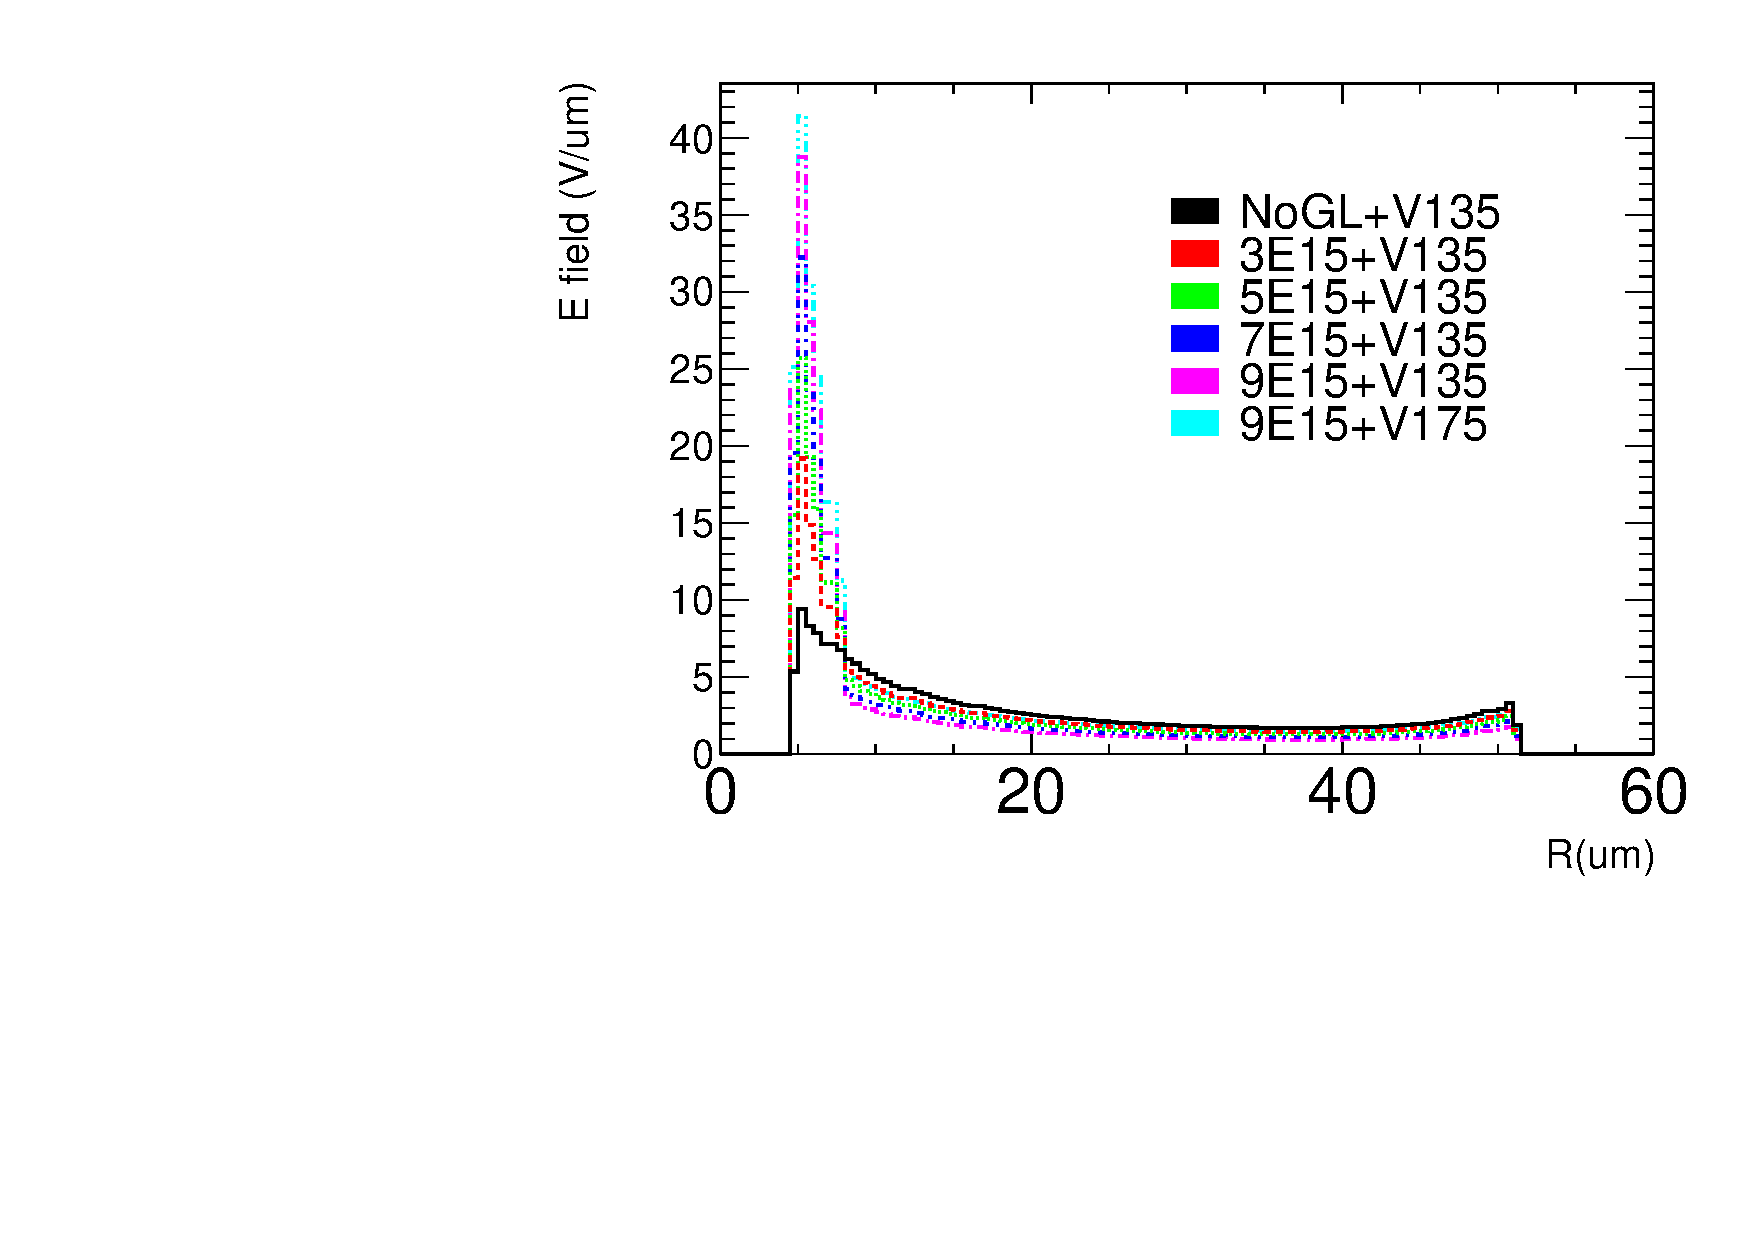
\includegraphics[width=0.35\textheight,keepaspectratio]{figures/Electric_field_IBLGAD5E_summary.pdf}
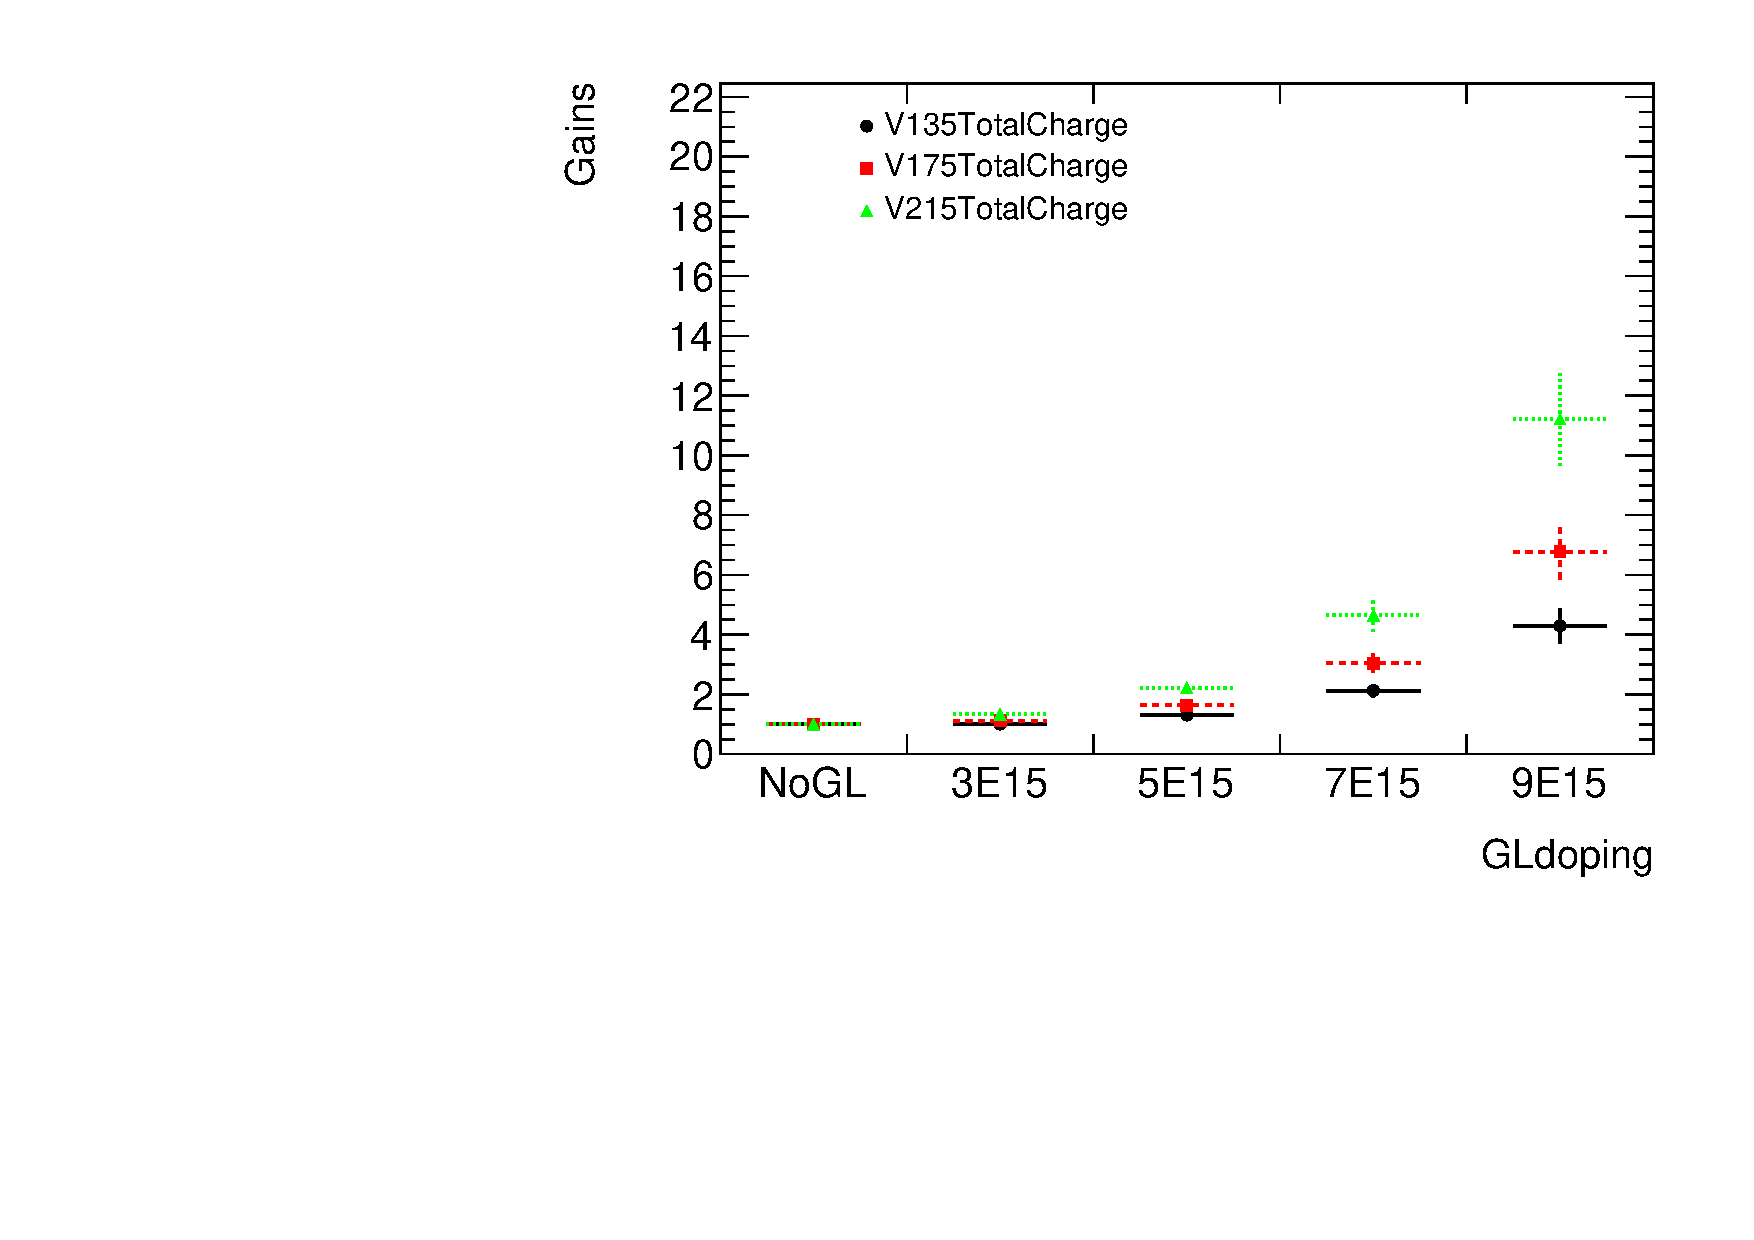
\includegraphics[width=0.35\textheight,keepaspectratio]{figures/Anatiming_timing3DIBLGAD5E_Plots_TotalChargeGLdoping.pdf}
\caption{The projection of the electric fields along the diagonal line between n+ and p+ electrodes (left) and 
the average charge collection gains for a MIP (right) as a function of GL doping densities and the bias voltages.~\label{fig:kdetgain}}
\end{center}
\end{figure}

\begin{figure}[hbtp]
\begin{center}
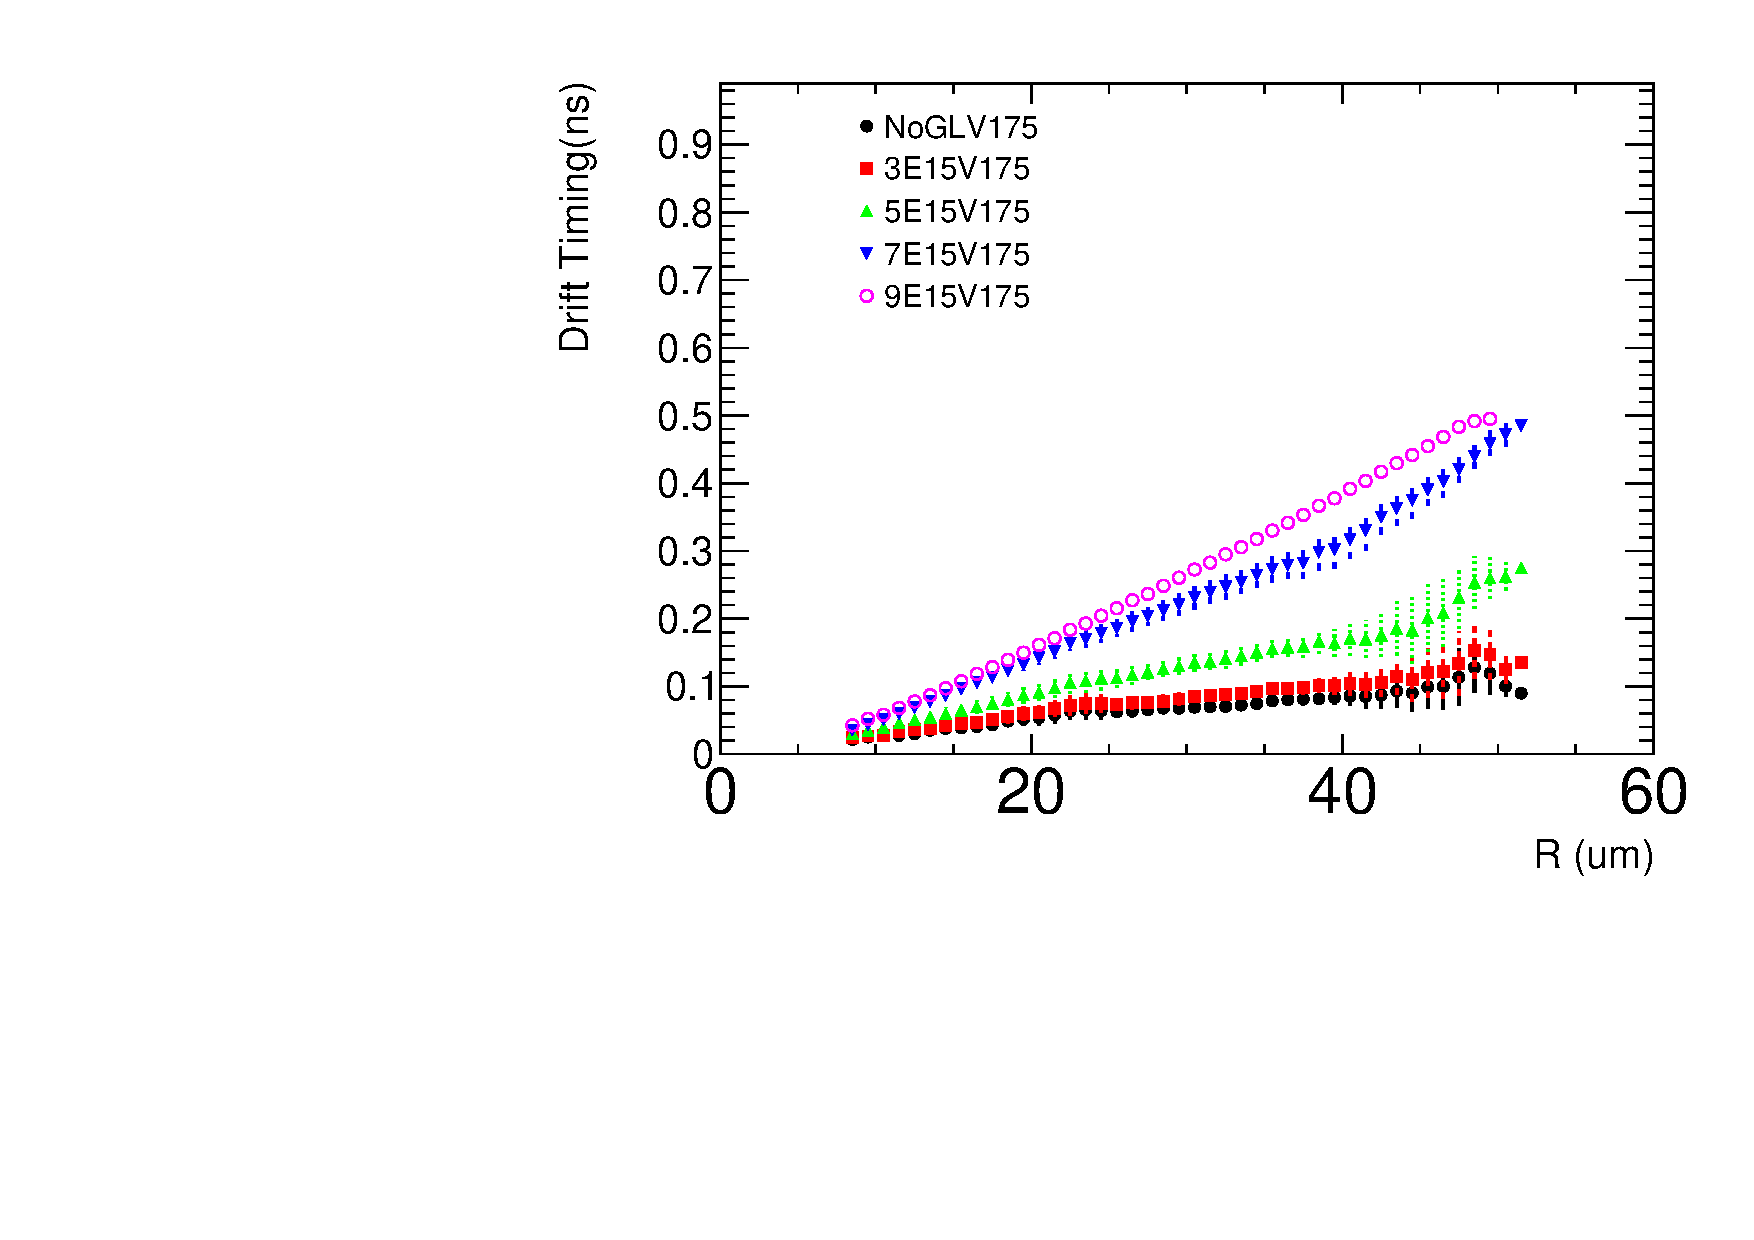
\includegraphics[width=0.25\textheight,keepaspectratio]{figures/Anatiming_timing3DIBLGAD5E_Plots_V175.pdf}
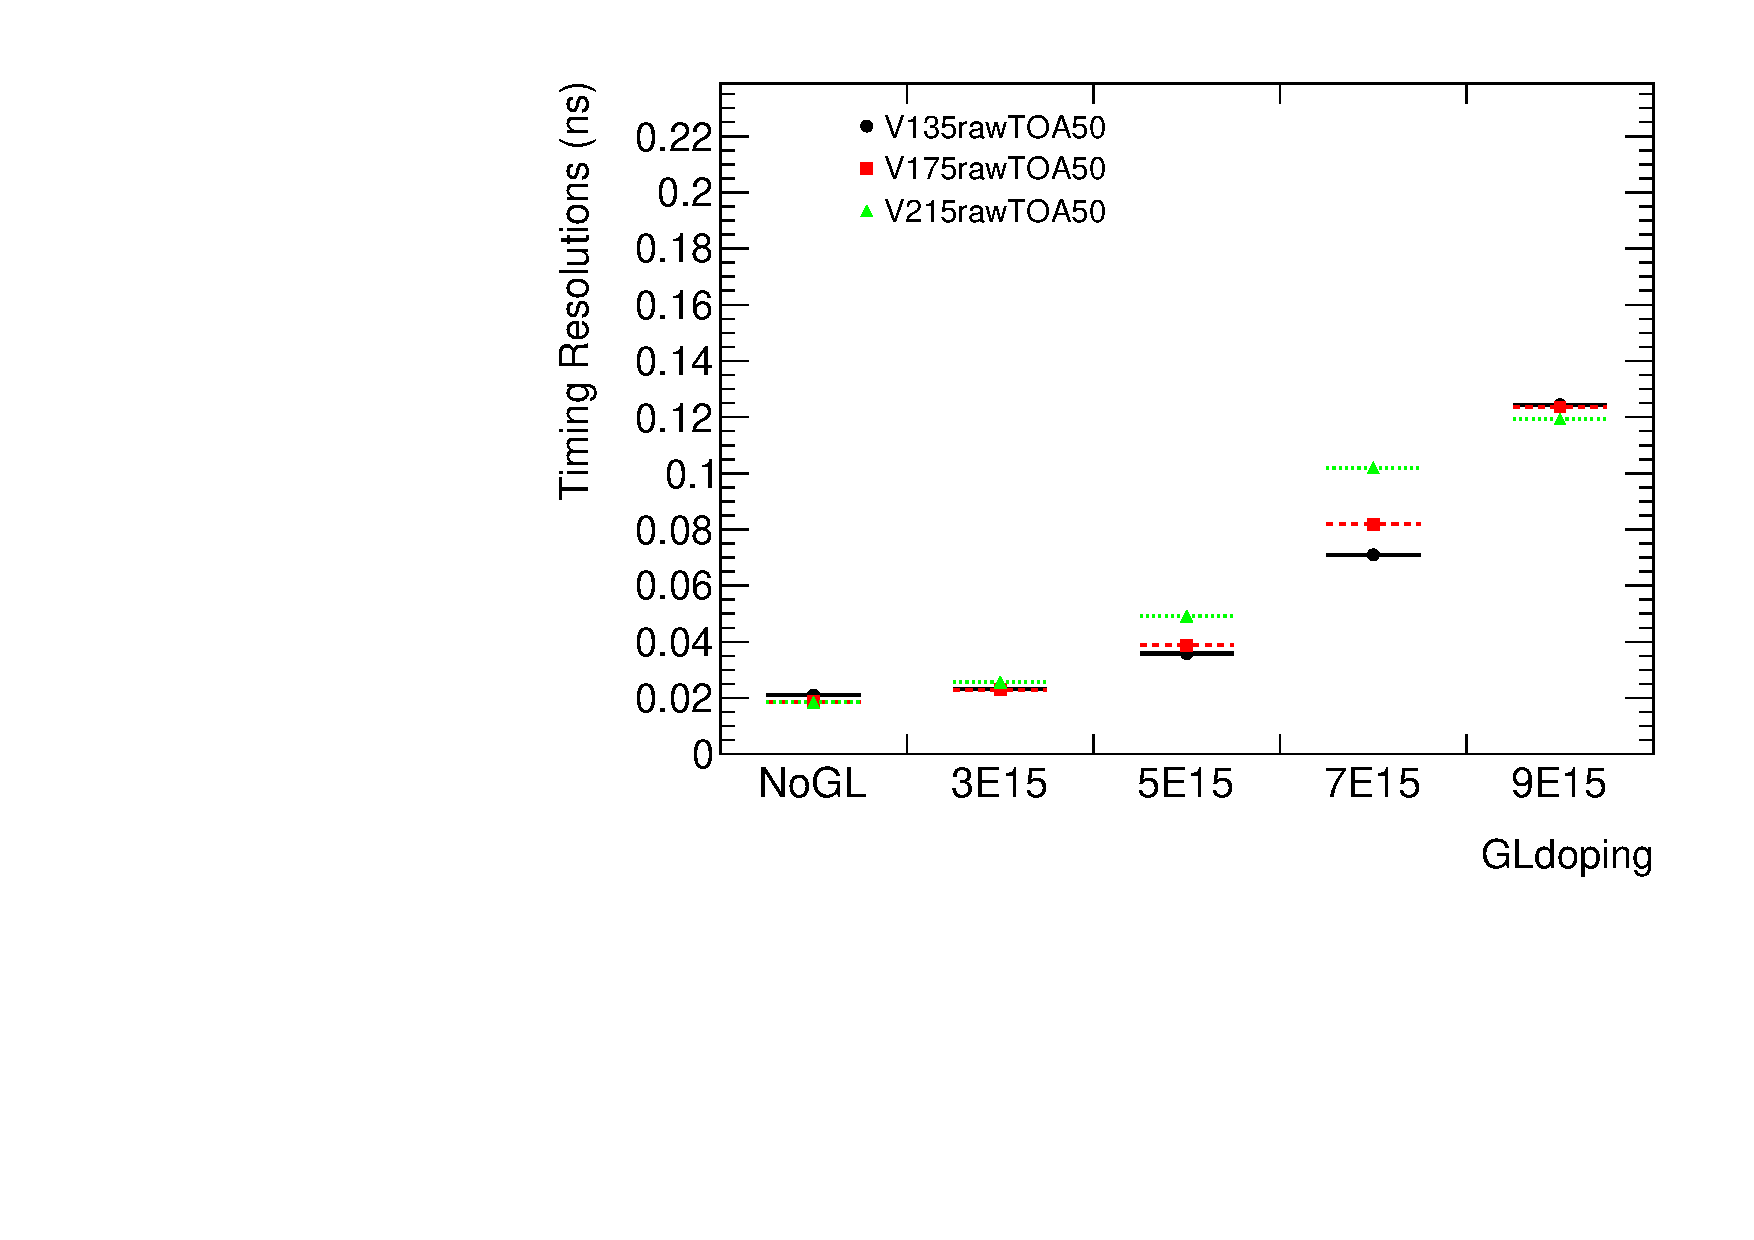
\includegraphics[width=0.25\textheight,keepaspectratio]{figures/Anatiming_timing3DIBLGAD5E_Plots_rawTOA50GLdoping.pdf}
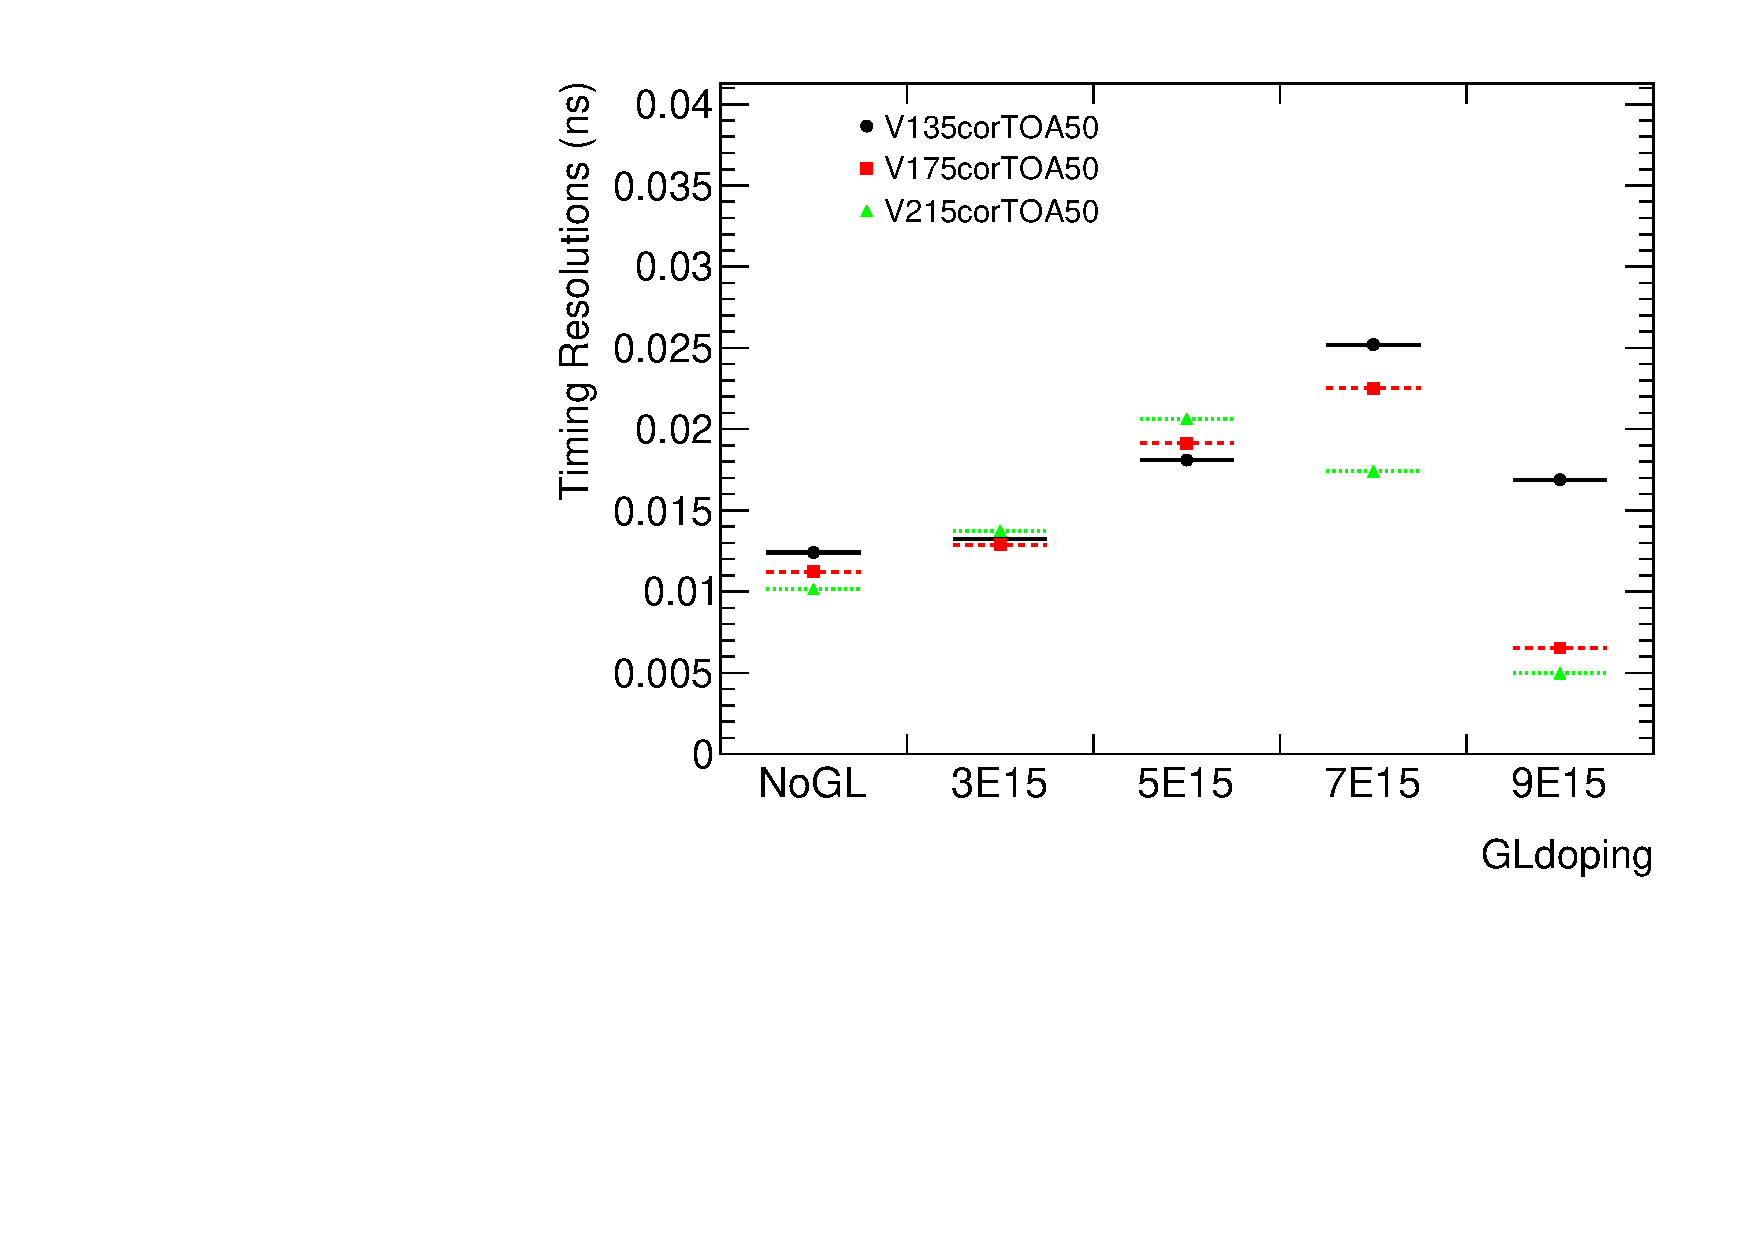
\includegraphics[width=0.25\textheight,keepaspectratio]{figures/Anatiming_timing3DIBLGAD5E_Plots_corTOA50GLdoping.pdf}
\caption{The drift-time (TOA50) as a function of drift distance from the n+ electrode (left); the average TOA50 before (middle) and 
after (right) the drift-time corrections.~\label{fig:kdettoa}}
\end{center}
\end{figure}

\section{Challengs} 

The 3D-LGAD sensor could be difficult to
produce in large-scale due to the challenges of properly doping the electrodes.
The electrodes are normally made by depositing the poly-silicon inside the holes and
they are doped by diffusion from solid or liquid source.
An alternative procedure is required to dope the gain layer properly. 

There are also significant challenges to develop the next generation of readout ASIC chips with
a pixel size of 50x50 $\mu m^2$ and a timing resolution of $\approx$~30~ps.
The current RD53 chip has a correct pixel size, but it has no proper
timing resolution. On the other hand, the ALTIROC chip designed for HGTD at ATLAS has
a timing resolution of 20~ps, but its pixel size is 1.3~mm x 1.3~mm,
too large for precision tracking~\cite{delaTaille:2018qap}.

\section{Conclusion}

In this study, we present some preliminary results on the 3D-LGAD sensor based TCAD simulation, which
could improve the signal-to-noise ratio to achieve a better timing resolution.
We aim to develop a truly 4-D silicon pixel detector with 3D sensor with both a spatial
resolution of $\approx 10~\mu m$ and a timing resolution of $\approx$30~ps
that  will open a new era for precision tracking, reducing pile-up
events and particle identification for the future colliding experiment.

\bibliographystyle{elsarticle-num}
\def\bibname{\Large\bf References}
\def\refname{\Large\bf References}
\pagestyle{plain}
\bibliography{IBL3DLGAD_NIM}

\end{document}
